%=============================================================================
\chapter{Fundamental Concepts and Methodologies in Swarm Control}\label{chap:fundamentals}
%=============================================================================

\section{Swarm Intelligence and Self-Organization}\label{sec:si}

Swarm intelligence (SI) is an artificial intelligence paradigm that explains how
large groups of simple agents with limited capabilities, solely through local
interactions and without centralized control, give rise to intelligent, robust,
flexible, and scalable behavior at the collective level \cite{bonabeau1999swarm}.

Self-organized natural phenomena in social insects---such as foraging by ants,
nest construction by termites, and collective migration---have inspired SI
methods that solve complex distributed problems through decentralized
decision-making and indirect coordination, which makes these methods attractive
for modern engineering systems \cite{garnier2007biological}.

\subsection{Definition and Concepts of Swarm Intelligence}

Swarm intelligence is an important branch of AI that studies the intelligence
emerging from the interactions of a large number of simple agents, and it
clearly illustrates the principle that ``the whole is greater than the sum of
its parts.'' Successful SI algorithms abstract the behaviors of social insects
into computational procedures and control laws and apply them to optimization,
decision-making, and distributed robotics. Emergent properties arise from
nonlinear local interactions and feedback, producing macroscopic patterns such
as trail networks, task allocation, and cooperative transport. These mechanisms
translate into decentralized control of robot swarms and are used for tasks such
as exploration, coverage, clustering/sorting, and construction/self-assembly
\cite{bonabeau1999swarm,bhowmick2024bio}.

\subsubsection{Decentralized and Self-Organized Problem Solving}

Decentralization means solving complex distributed problems without a central
controller or a global state, with sensing, actuation, and communication
distributed among the agents to improve robustness and scalability \cite{bonabeau1999swarm}.

Self-organization is the spontaneous formation of ordered global patterns from
many local interactions based on simple rules; the environment often serves as
an external memory and communication medium for these indirect interactions
\cite{garnier2007biological}.
\begin{itemize}
  \item \lead{Stigmergy (indirect coordination)} Stigmergy is coordination
        through modifications of the environment: agents ``write'' cues (e.g.,
        pheromone-like markers) that later ``reader'' agents use as the basis
        for their actions, which enables delayed, scalable, and decentralized
        communication.
  \item \lead{Practical implementations} These include virtual pheromones,
        deployed markers with simulated diffusion, robots that deliberately act
        as stationary beacons or repeaters for a while, and software agents that
        read from and write to a shared state \cite{sahin2005swarm}.
\end{itemize}

\subsection{Principles of Self-Organization and Stigmergy}

Self-organization explains the emergence of macroscopic order solely from local
agent--agent and agent--environment interactions, without central control and
without explicit global templates \cite{bonabeau1999swarm,garnier2007biological}. It rests on four fundamental
principles:
\begin{itemize}
  \item \lead{Positive feedback} Recruitment and reinforcement amplify partially
        useful solutions and create a snowball effect (e.g., trail reinforcement
        in ants).
  \item \lead{Negative feedback} Resource depletion, evaporation, competition, or
        saturation stabilize the patterns and prevent runaway dynamics.
  \item \lead{Amplification of fluctuations} Individual randomness seeds
        exploration and enables the discovery of new solutions (e.g., new food
        sources).
  \item \lead{Multiple interactions} An abundance of local interactions creates
        the correlation and cohesion needed for stable macroscopic structures.
\end{itemize}

\subsubsection{Indirect Coordination through Environmental Cues}

Coordination can be direct (physical or visual contact) or indirect, through
modifications of the environment; the latter is an instance of stigmergy. The
environment acts as a shared, persistent external memory, allowing robots with
local sensing to exchange information asynchronously and reach collective goals
without global knowledge \cite{bonabeau1999swarm,garnier2007biological}.

Local decisions based on sensed cues drive global organization and allow agents
with limited perception to build trails, allocate tasks, and construct
structures. This delayed, cue-based communication improves scalability and
robustness against failures or communication loss in large swarms \cite{bonabeau1999swarm,garnier2007biological}.

\subsubsection{Stigmergy in Natural and Artificial Swarms}

In natural systems, Grass\'e introduced stigmergy to explain nest reconstruction
in termites: each building action turns the local configuration into a new
stimulus that coordinates subsequent actions without any supervisor
\cite{bonabeau1999swarm}.

Ant foraging is another important example: pheromone deposition and evaporation,
acting as positive and negative feedback, give rise to self-organized trail
networks that discover and reinforce the shortest paths under geometric
constraints \cite{garnier2007biological}.

There are two types of stigmergy:
\begin{itemize}
  \item \lead{Quantitative (continuous)} Responses vary with the intensity of the
        stimulus (e.g., pheromone concentration), which explains pillar
        construction and trail reinforcement.
  \item \lead{Qualitative (discrete)} Distinct categories of stimuli trigger
        different actions, as in paper-wasp nest construction guided by local
        cell configurations \cite{bonabeau1999swarm}.
\end{itemize}

Artificial implementations of stigmergy in swarms include:
\begin{itemize}
  \item \lead{Virtual pheromones} Software or field representations simulate
        deposition, diffusion, and evaporation in order to form trails, provide
        coverage, and prioritize regions.
  \item \lead{Embedded media} Smart environmental beacons or markers encode
        stigmergic information and simulate diffusion to provide scalable
        guidance.
  \item \lead{Physical agents as the medium} Some robots become stationary relays
        or anchors and provide local memory and navigation cues in large swarms.
  \item \lead{Software agents and shared states} Agents write to and read from a
        shared layer or map and use it as an external memory for indirect
        coordination \cite{bonabeau1999swarm,sahin2005swarm}.
\end{itemize}

A canonical mathematical model of trail-based stigmergy is as follows. Ants
choose between two branches with a pheromone-weighted probability $p(C_i)$, and
the pheromone dynamics, with evaporation and deposition, lead to a bifurcation
from symmetric to asymmetric traffic above a critical flux \cite{garnier2007biological}. The path
choice is given by
\begin{equation}
  p\left(C_i \mid C_1, C_2\right)
    = \frac{(k + C_i)^{\alpha}}{(k + C_1)^{\alpha} + (k + C_2)^{\alpha}},
    \qquad i = 1, 2,
  \label{eq:trail-choice}
\end{equation}
where $k$ and $\alpha$ depend on the species and the experimental setup. The
pheromone evolves according to
\begin{equation}
  \frac{dC_i}{dt} = \Phi\, p\left(C_i \mid C_1, C_2\right) - \mu\, C_i,
    \qquad i = 1, 2,
  \label{eq:pheromone-dynamics}
\end{equation}
where $\Phi$ is the incoming flux and $\mu$ is the evaporation rate; this leads
to multiple equilibria and to symmetry breaking beyond a critical value of
$\Phi$.

\begin{figure}[htbp]
  \centering
  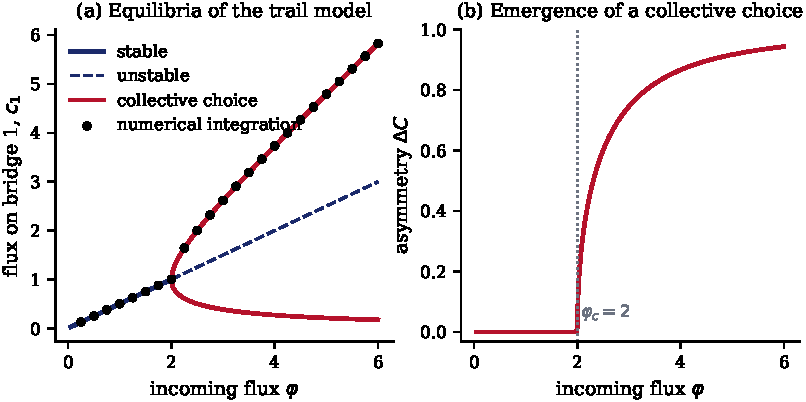
\includegraphics[width=0.58\linewidth]{collective-choice-flow}
  \caption{Flow analysis and the emergence of a collective choice.}
  \label{fig:collective-choice}
\end{figure}

\Cref{fig:collective-choice} shows the traffic flows that produce a collective
choice as a function of the individual deposition amount~$q$. The collective
response (the vertical axis) is indicated by the flow becoming asymmetric over
the two bridges, i.e.,
\begin{equation}
  \Delta C = \frac{\left|C_1 - C_2\right|}{C_1 + C_2}.
  \label{eq:asymmetry}
\end{equation}
A value of $\Delta C > 0$ indicates the emergence of a collective choice.

%-----------------------------------------------------------------------------
\section{Control Architectures for Swarm Robotics}\label{sec:control-architectures}

Control architectures in swarm robotics are designed to achieve robust,
scalable, and flexible collective behavior; they emphasize decentralized
decision-making, lightweight local communication, and formal mechanisms for
convergence and safety in large groups of robots. The central challenge in
swarm control design is that the control paradigm determines how information
flows among the agents and how local interactions produce reliable macroscopic
performance under uncertainty and failures \cite{hamann2018swarm}.

Unlike classical robotics, swarm control favors distributed, self-organized
schemes over monolithic global supervisors, in order to avoid bottlenecks,
single points of failure, and scalability problems with hundreds or thousands of
agents \cite{dias2021swarm}.

\subsection{Decentralized Control}

Decentralized control is the cornerstone of swarm robotics: each robot runs a
simple, autonomous controller that relies on local sensing and neighborhood
exchanges, and macroscopic performance emerges from concurrent local decisions
without a central coordinator \cite{hamann2018swarm,nguyen2024swarm}.

\subsubsection{Local Decision-Making and Adaptability}

In decentralized architectures, each agent perceives only its own
neighborhood, applies local rules, and updates in parallel with its peers; in
this way, behaviors such as flocking, pattern formation, and exploration emerge
without the need for a map or for broadcasting a global state \cite{hamann2018swarm}.
Locality enables rapid adaptation: when the environment or the mission changes,
the agents immediately adapt to the new local cues and drive a coherent
macroscopic reconfiguration without global commands \cite{dias2021swarm}.

A typical local control law for agent $i$ is based on the differences with its
neighbors:
\begin{equation}
  \dot{x}_i = \sum_{j \in \mathcal{N}_i} a_{ij}\,\left(x_j - x_i\right),
  \label{eq:consensus-agent}
\end{equation}
which can be written in vector form as
\begin{equation}
  \dot{x} = -L x,
  \label{eq:consensus-vector}
\end{equation}
where $L$ is the graph Laplacian; convergence is guaranteed under standard
connectivity assumptions \cite{hamann2018swarm}.

Distributed flocking, by combining the simple rules of separation, alignment, and
cohesion, or by imposing geometric constraints, maintains distances, headings,
and shapes using only neighbor data and enables robust motion through unknown
environments \cite{lee2018realtime}.

\subsubsection{Distributed Algorithms and Scalability}

Distributed swarm algorithms emphasize simplicity, locality, robustness, and
parallelism, so that the complexity per robot stays low and performance is
preserved as the team grows \cite{nguyen2024swarm}.

Centralized schemes often suffer from channel congestion and high latency,
whereas distributed protocols naturally balance the load, tolerate faults, and
exploit the concurrency of sensing and actuation \cite{hamann2018swarm}.
\begin{itemize}
  \item \lead{Simplicity and finite state machines} Controllers are often finite
        state machines (FSMs) or short reactive chains, so that their timing
        remains predictable \cite{hamann2018swarm}.
  \item \lead{Local-only communication} Neighbor-to-neighbor exchange preserves
        scalability and avoids saturating a global channel, while still enabling
        consensus, formation, and task allocation over graphs \cite{liu2018virtual}.
  \item \lead{Dynamic membership} Agents may join or leave; the protocols are
        recomputed with the current neighbors and have no hard dependence on
        specific members \cite{dias2021swarm}.
\end{itemize}

\subsubsection{Consensus Principles}

Consensus is the agreement of robots on shared variables---such as reference
frames, headings, goals, virtual leaders, or shape parameters---through local
exchanges over a graph with adjacency matrix $A$ and Laplacian $L$.
Continuous-time average consensus follows $\dot{x} = -Lx$, and its discrete-time
counterpart $x_{k+1} = (I - \varepsilon L)\,x_k$ with step size $\varepsilon$
converges if the graph is connected and the spectral conditions hold \cite{hamann2018swarm}.

Whether in direct, message-based modes or in indirect modes based on density or
motion, consensus is reached on choices such as waypoints or formation branches,
reflecting collective decision-making \cite{hamann2018swarm}.

Practical controllers estimate distributed quantities using local filters,
event-triggered updates, or time-varying weights, in order to reduce bandwidth
and to track changing goals stably and quickly \cite{liu2018virtual}.

An example of event-triggered multi-robot control based on the adjacency matrix
$A = [a_{ij}]$ is
\begin{equation}
  u_i(t) = \sum_{j} a_{ij} \Bigl[\alpha\bigl(x_j(t_j^{s}) - x_i(t_i^{s})\bigr)
           + \beta\bigl(v_j(t_j^{s}) - v_i(t_i^{s})\bigr)\Bigr],
  \label{eq:event-triggered}
\end{equation}
which uses a triggering condition $g_i(t) > 0$ so that each robot updates and
transmits only when necessary, and which guarantees position--velocity consensus
through Lyapunov analysis \cite{liu2018virtual}.

\subsection{Behavior-Based Control Methods}

Behavior-based control (BBC) realizes swarm intelligence through bottom-up
reactive behaviors rather than global plans, keeping the system simple, robust,
and responsive in unknown or dynamic environments \cite{hamann2018swarm}.

BBC is aligned with local sensing/actuation and emergent coordination, which are
hallmarks of scalable swarm operation. Subsumption-style layering prioritizes
behaviors (e.g., obstacle avoidance above exploration): the behaviors run
concurrently, but higher-priority behaviors suppress lower-priority ones and
release them once the stimulus disappears. Iterative refinement at the robot
level---tuning behaviors and thresholds---produces reliable collective patterns
without a global model or explicit global synchronization \cite{nguyen2024swarm}.

\subsubsection{Reactive Behaviors for Emergent Intelligence}

Reactive controllers map the current sensor inputs and a minimal internal state
to actions through condition--action rules and avoid complex world models, so
that they remain replicable across large teams \cite{hamann2018swarm}. Emergent behaviors
such as flocking, dispersion, trail formation, and collective decision-making
arise from many local interactions rather than from a single global planner
\cite{lee2018realtime}.

Artificial potential fields (APFs) superimpose attractive forces toward goals and
repulsive forces from obstacles and peers to provide safe distributed navigation
without global supervision, although parameter tuning and local minima require
care.

\subsubsection{Finite State Machines in Controllers}

FSMs are widely used in swarm controllers: states encapsulate behaviors, and
transitions are triggered by sensor events, timers, or messages, which ensures
predictable responsiveness with a simple architecture \cite{hamann2018swarm}. Probabilistic
FSMs (PFSMs) add stochastic transitions to model noise and variability and
facilitate the analysis of convergence and robustness in aggregation, chaining,
or allocation tasks \cite{hamann2018swarm}.

\subsubsection{Response Threshold Models}

Response threshold models link an agent's probability of switching tasks to the
intensity of a stimulus, producing decentralized and flexible task allocation in
which task sequencing emerges from the accumulation of collective stimuli
\cite{hamann2018swarm}. The standard nonlinearity is
\begin{equation}
  p(s) = \frac{s^{\beta}}{s^{\beta} + \theta^{\beta}},
  \label{eq:response-threshold}
\end{equation}
where $s$ is the stimulus, $\theta$ is the threshold, and $\beta$ controls the
sensitivity. As $s$ exceeds $\theta$, the probability of acting rises sharply,
and coordination emerges without an explicit leader.

\subsection{Hybrid Control Methods}

Hybrid controllers combine behavior-based control with systems-theoretic
guarantees to handle missions that require both fast local responses and
guaranteed macroscopic performance \cite{hamann2018swarm}. A common pattern embeds reactive
rules within a statistical or model-based regulator that governs swarm-level
quantities (e.g., the mean position or the density variance), thereby preserving
autonomy while constraining the macroscopic behavior \cite{hamann2008space}.

This synthesis retains robustness and scalability while achieving explicit
objectives such as tracking, containment, and safety margins through provable
controllers layered around the reactive behaviors.

\subsubsection{Combining Behavior-Based and Systems-Theoretic Approaches}

The goal is to retain the qualitative strengths of BBC---simplicity, robustness,
and fast reaction---while adding formal control to regulate collective metrics
and stability \cite{hamann2018swarm}.

Statistical or macroscopic controllers can constrain the swarm's center of mass
and dispersion, while reactive layers ensure collision avoidance, obstacle
negotiation, and local safety, thus reconciling global guarantees with local
autonomy \cite{hamann2008space}.

Formal tools include Lyapunov functions, graph-theoretic convergence results,
and density-based partial differential equation (PDE) formulations for
quantifying and bounding macroscopic performance under distributed execution
\cite{hamann2018swarm}.

\subsubsection{Applications: Multi-AUV Underwater Missions}

Hybrid control excels underwater, where uncertain currents, limited
communication, and safety-critical sensing require both local reaction and
macroscopic coordination for cooperative target hunting or survey coverage
\cite{liu2018virtual}.

Event-triggered and consensus-based schemes reduce bandwidth while maintaining
formation and tracking, and reactive potential fields provide on-the-spot
avoidance of obstacles and hazards \cite{liu2018virtual}.

In such implementations, the macro layer regulates group objectives (e.g., the
mean trajectory of the formation), while the micro layers execute avoidance,
separation, and target pursuit, so that the autonomy and survivability of each
autonomous underwater vehicle (AUV) are preserved.

A worked example of this layering, cooperative target hunting by a team of
AUVs with an improved potential field, is described in \cref{sec:potential-fields}
\cite{ge2018multi}.

\subsection{Virtual Structure and Virtual Linkage Approaches}

Formation control can be framed as leader--follower, behavior-based, or virtual
structure (VS) control. The virtual linkage (VL) approach generalizes VS to allow
precise control with reconfiguration through virtual joints and links. VL treats
the formation as a mechanical structure of virtual links connected by joints
whose angles determine the shape of the pattern, and it enables reshaping by
controlling the trajectories of these angles \cite{liu2018virtual}.

\subsubsection{Virtual Linkage and Degrees of Freedom}

In VL, the desired shape is parameterized by the virtual joint angles
$\Theta_d$, and the number of joints equals the number of degrees of freedom
available for reconfiguring the pattern; adding an expansion/contraction vector
$\lambda_d$ scales the link lengths for passing through narrow passages. Because
the robots follow only local virtual-linkage references, reshaping is achieved
by broadcasting a small set of parameters to a few link-level controllers, which
reduces communication compared with recomputing the slot of every member
\cite{liu2018virtual}.

VL decouples precise control from global design, offers a compact command space
for frequent changes of shape, and keeps execution distributed at the robot
level. \Cref{fig:virtual-linkage} illustrates how a virtual linkage works.

\begin{figure}[htbp]
  \centering
  \tikzfigure[0.55\linewidth]{virtual-linkage}
  \caption{A mechanical linkage and its virtual counterpart, the virtual linkage
           (redrawn after \cite{liu2018virtual}).}
  \label{fig:virtual-linkage}
\end{figure}

%-----------------------------------------------------------------------------
\section{Communication and Sensing in Swarms}\label{sec:communication}

Communication and sensing are the main channels through which collective
intelligence manifests itself in swarms; local exchange and interaction mirror
the decentralized organization found in nature. The chosen control architecture
fixes the topology of information exchange and hence the performance, so
reliable, fault-tolerant communication is essential for effective coordination
at scale \cite{ge2018multi}.

\subsection{Local Interactions and Limited Communication}

Swarm controllers place decision-making at the agent level and, with simple
computation and minimal sensors on each robot, achieve scalability, robustness,
and flexibility through parallel, neighbor-based interactions. This design
removes any dependence on a global state and keeps working in the presence of
motion, topology changes, and partial failures \cite{dias2021swarm}.

\subsubsection{Local Sensing Capabilities}

Swarm robots are usually homogeneous and resource-constrained, so sensing is
deliberately local and minimal to keep cost and energy consumption low while
still enabling distributed behaviors. Consequently, each robot acts on
instantaneous observations and simple rules, and the range and bearing to nearby
neighbors are vital \cite{dias2021swarm}.
\begin{itemize}
  \item \lead{The need for local sensing} Agents perceive nearby robots and
        obstacles and act autonomously using only these measurements and concise
        rules, which often involve estimating the distances to neighbors for the
        interaction rules.
  \item \lead{Sensor types} Common modalities include proximity and range sensing
        (infrared (IR), ultrasonic), cameras and light sensors, inertial
        measurement units (IMUs), microphones, and simple environmental sensors.
        Very small platforms use IR LEDs and photodiodes for local communication
        and relative localization, and the Kilobot uses downward-facing IR
        reflected off the floor for limited-range communication and localization.
  \item \lead{Purpose} Local sensing makes it possible to follow local rules and
        interact with neighbors, which is essential for decentralized
        coordination and the emergence of group behavior \cite{hamann2018swarm}.
\end{itemize}

\subsubsection{Challenges in Predicting Simultaneous Interactions}

Decentralized swarms face predictability challenges because abundant local
interactions create nonlinear, emergent dynamics that are difficult to control
and predict in advance. This complexity stems from micro-to-macro coupling, in
which macroscopic behavior emerges from microscopic decisions made under limited
information and a changing topology \cite{ge2018multi,hamann2018swarm}.
\begin{itemize}
  \item \lead{Unpredictable emergence} Undesired global patterns can emerge from
        large numbers of simultaneous local interactions, complicating formal
        guarantees and certification.
  \item \lead{Cognitive load} The cognitive difficulty for a human operator does
        not remain a constant $O(1)$; dependencies and incomplete information
        under bandwidth and latency constraints increase the supervision burden.
  \item \lead{Topology dependence} Motion reshapes the graph and risks
        fragmenting it into disconnected components, unless the algorithms
        preserve connectivity and robustness under dynamic neighbor sets.
  \item \lead{Information propagation} Building global maps or shared situational
        awareness from local observations is constrained by short-range,
        limited-bandwidth links and requires efficient multi-hop dissemination in
        highly dynamic networks.
\end{itemize}

\subsubsection{Short-Range Communication}

Swarm design deliberately restricts communication to short ranges to preserve
scalability and robustness by avoiding channel saturation and single points of
failure. Local links enable massive parallelism and redundancy and keep the
hardware of each robot simple and inexpensive \cite{dias2021swarm}.
\begin{itemize}
  \item \lead{Scalability constraint} Global channels scale poorly as the team
        grows, so protocols enforce neighbor-only exchange to keep communication
        costs bounded and decentralized.
  \item \lead{Communication modalities} Both explicit links (peer-to-peer radio)
        and implicit ones (stigmergic or environmental cues, physical contact)
        support distributed coordination under local rules.
  \item \lead{Radio frequency (RF)} IEEE 802.15.4-class radios on platforms such
        as the e-puck are often configured with power control for very short
        ranges (up to a few tens of centimeters) to enforce locality \cite{liu2018virtual}.
  \item \lead{Infrared (IR)} Short-range messaging and proximity sensing,
        including mutual ranging and neighbor discovery, as in the
        s-bot/Swarm-bot systems \cite{sahin2005swarm,liu2018virtual}.
  \item \lead{Sound/ultrasonic} Acoustic links aid localization and messaging and
        can be combined with RF triggering for GPS-free distributed operation on
        land and underwater; the e-puck, for example, carries microphones and a
        speaker that can be used for acoustic messaging \cite{sahin2007swarm}.
\end{itemize}

\subsection{Communication Protocols and Network Topology}

Swarm performance depends strongly on the communication architecture and on the
network topology it induces; together, they determine how information flows, how
quickly consensus forms, and how resilient coordination is to faults. The
co-design of protocol and topology must account for motion-induced changes and
bandwidth constraints in order to maintain stability and throughput \cite{ge2018multi}.

\subsubsection{Decentralized Communication Protocols}

Decentralized protocols allow robots to exchange data without a central broker,
producing robust, scalable, low-latency coordination. The categories include
direct messaging, indirect stigmergy, and direct physical interaction, which are
often combined for redundancy and adaptability \cite{hamann2018swarm,dias2021swarm,ge2018multi}.
\begin{itemize}
  \item \lead{Direct peer-to-peer communication} Explicit exchange of states,
        events, or votes reduces latency and enables rapid reactions to local
        contingencies.
  \item \lead{Indirect communication (stigmergy)} Agents leave environmental
        markers that shape subsequent decisions, providing an inexpensive,
        delay-tolerant flow of information.
  \item \lead{Direct interaction} Physical contact or force sensing conveys local
        state cues and constraints and is useful in tight formations and
        cooperative manipulation.
  \item \lead{Design goals} Local decision-making with adaptive protocols,
        multipath redundancy, and distributed communication functions reduces
        single points of failure and preserves functionality under partial
        outages.
\end{itemize}

\subsubsection{Graph Theory and Network Structure}

Graph theory models robots as nodes and communication links as edges, enabling
analysis based on the adjacency matrix $A$ and the Laplacian $L = D - A$ (where
$D$ is the degree matrix) to support convergence proofs for distributed
controllers. The choice of graph and its connectivity determine the stability
and convergence rates of consensus, formation, and distributed estimation
\cite{hamann2018swarm}.
\begin{itemize}
  \item \lead{Graph types} Undirected graphs model bidirectional exchange and
        directed graphs (digraphs) model one-way flow; the spectral properties of
        $L$ shape the convergence and robustness margins.
  \item \lead{Proximity graphs} The limited sensing and communication range
        induces proximity topologies such as the $r$-disk graph
        $G_{\mathrm{disk}}(r)$, in which an edge exists between two robots that
        are closer than $r$.
  \item \lead{Leader--follower structure} A leader guides the collective motion
        and the followers track it using the leader's state and data from their
        neighbors; convergence in directed networks usually requires a directed
        spanning tree rooted at the leader.
\end{itemize}

\subsubsection{Network-Theoretic Approach to Information Flow}

The network-theoretic perspective views the signaling network of a swarm as a
temporal, adaptive system whose topology co-evolves with the motion of the
agents, coupling communication and control. Information constraints---a limited
capacity $C$ and bandwidth $B$---bound the achievable performance and call for
bandwidth-aware coordination and compression \cite{hamann2008space}.
\begin{itemize}
  \item \lead{Structural properties} Many biological and engineered swarms exhibit
        small-world traits---short paths and high clustering---which support the
        fast and robust propagation of behavioral signals.
  \item \lead{Network controllability} Analysis can identify the minimal set of
        driver agents needed to steer the swarm dynamics and can inform the
        placement of leaders, beacons, or gateway nodes.
\end{itemize}

\subsection{Sensor Models and Data Acquisition}

Sensing, alongside actuation and computation, is a core subsystem; context
awareness is obtained by fusing environmental and inter-agent measurements,
including communication signals interpreted as sensors of the network state. The
key challenge is to fuse heterogeneous, local sensors into robust cooperative
behaviors and shared maps under tight resource constraints \cite{hamann2018swarm,dias2021swarm}.

\subsubsection{Sensor-Based Scene Understanding}

Scene understanding combines representation and data association to produce
actionable context from on-board measurements. Three complementary levels of
representation are common in swarms with heterogeneous payloads and different
roles \cite{dias2021swarm}:
\begin{itemize}
  \item \lead{Appearance level} Local and global visual features support state
        estimation and visual place recognition for lightweight localization.
  \item \lead{Geometry level} LiDAR and RGB-D sensors provide 3-D points and
        depth; RGB-D is sensitive to lighting, whereas LiDAR is costly and heavy,
        which justifies deploying them selectively in mixed swarms.
  \item \lead{Semantic level} Object detection, multi-target tracking, and
        semantic segmentation improve navigation and make simultaneous
        localization and mapping (SLAM) robust to dynamic changes.
  \item \lead{Output artifacts} Semantic local maps and scene graphs provide
        high-level constraints for distributed localization and cooperative
        planning.
\end{itemize}

%-----------------------------------------------------------------------------
\section{Basic Concepts of Path Planning}\label{sec:path-planning-basics}

Path planning is a fundamental problem in robotics and autonomous systems because
it provides the high-level decision-making layer that selects a continuous
sequence of spatial waypoints for the robot to follow, and it directly affects
autonomy, safety, and mission efficiency. In swarm settings, path planning is
intertwined with the decentralized control and communication layers, and it
determines strategic routes that respect local sensing limitations while
optimizing global mission criteria such as time, energy, and robustness
\cite{nguyen2024swarm}.

\subsection{Definition of Path Planning}

Path planning is the problem of computing a feasible---and preferably
optimal---path that moves a robot from an initial state to a goal state in an
environment while respecting geometric, kinematic/dynamic, and safety
constraints. As the field has matured, the goal has shifted from finding ``any
path'' to finding multi-criteria optimal paths that reduce travel time, energy
consumption, and risk, while improving smoothness and robustness for real-world
deployments \cite{nguyen2024swarm}.

\subsubsection{Generating Collision-Free Paths}

A fundamental requirement is collision avoidance: the path must avoid static and
moving obstacles and maintain safety margins along its entire length. In the
configuration-space formulation, complex robot shapes are handled by
``inflating'' the obstacles or ``shrinking'' the robot to a point, so that
collision tests reduce to point-in-free-space checks and an efficient search over
admissible nodes and edges becomes possible \cite{hamann2018swarm}.

Once path planning has delivered a collision-free geometric path, motion planning
assigns time-parameterized velocity and acceleration profiles $v(t)$ and $a(t)$
that are consistent with the dynamic constraints, so that the path is tracked
smoothly and safely. Geometric safety can be enforced by inflating the obstacles
by the robot's footprint, which turns robot--obstacle interference into the
separation of a point from the inflated obstacles in the configuration space
\cite{hamann2018swarm,nguyen2024swarm}.

A typical tracking pipeline optimizes a timing law $s(t)$ along the curve
$\gamma(s)$ so that the bounds $\|\dot{\gamma}\| \le v_{\max}$ and
$\|\ddot{\gamma}\| \le a_{\max}$ are respected, thereby separating spatial
feasibility from dynamic feasibility for embedded controllers \cite{nguyen2024swarm}.

\subsubsection{A Constrained Optimization Problem}

Path planning is a constrained optimization search in which the objective may
combine distance, time, smoothness, energy, and robustness, while feasibility
must respect kinematic, dynamic, and safety constraints; many formulations are
NP-hard in the general case. Multi-objective criteria are common in multi-robot
systems and require Pareto reasoning or scalarization to balance conflicting
objectives, such as the shortest time versus the lowest energy or the largest
safety margin \cite{hamann2018swarm,nguyen2024swarm}.

A representative cost function is
\begin{equation}
  J(\gamma) = \alpha_1 L(\gamma) + \alpha_2 T(\gamma) + \alpha_3 S(\gamma)
              + \alpha_4 E(\gamma),
  \label{eq:cost-function}
\end{equation}
where $L$ is the length, $T$ is the travel time, $S$ is a surrogate for
smoothness such as curvature or jerk, and $E$ is the energy; the coefficients
$\alpha_i$ are tuned to the mission requirements. Swarm intelligence methods such
as PSO and ACO are widely used to approximate global optima under complex
constraints in high-dimensional configuration spaces or dynamic environments,
often smoothing the candidate paths with B-splines to respect nonholonomic
constraints \cite{panigrahi2011handbook}.

\subsection{Global versus Local Planning}\label{sec:global-local}

Planners are classified by the scope of their information: global planners
assume a known map and compute the path from start to end, whereas local
planners act reactively and rely on real-time sensing to cope with unknown or
dynamic obstacles. Practical systems are generally hybrid: global paths serve as
a prior, while local planners ensure safety and reactivity when the map is
incomplete or changes rapidly \cite{hamann2018swarm,nguyen2024swarm}.

\subsubsection{Global Planning}

Given a prior map, global planning computes the complete optimal path from the
origin to the destination, either by discretizing the free space and solving a
graph search or by sampling-based planning that efficiently captures the
connectivity of the space. Classical graph methods such as Dijkstra's algorithm
and \Astar{} guarantee optimality on weighted grids or roadmaps under admissible
heuristics, but they incur replanning overhead when the environment changes
\cite{hamann2018swarm}.

\Astar{} uses a heuristic $h(n)$ with $f(n) = g(n) + h(n)$, and optimality is
preserved when $h$ is admissible and consistent; this is effective for static
maps, but updates are needed when obstacles move. Sampling-based planners such as
the probabilistic roadmap (PRM) and the rapidly-exploring random tree (RRT)
family capture the connectivity of the free space without exhaustive gridding and
scale to high-dimensional configuration spaces, although in their basic forms
they rely on asymptotic rather than exact optimality \cite{nguyen2024swarm}.

\subsubsection{Local Planning}

Local planners rely on on-board sensing to generate admissible motions in real
time and, with minimal model assumptions, focus on obstacle avoidance and
progress toward the goal. Reactive approaches such as artificial potential fields
superimpose an attractive potential toward the goal and repulsive potentials
around the obstacles, providing low-computation navigation; without enhancements,
however, they suffer from local minima and oscillation \cite{bhowmick2024bio}.

The APF law takes the form
\begin{equation}
  U(x) = U_{\att}(x) + U_{\rep}(x),
  \label{eq:apf-basic}
\end{equation}
with the control $u(x) = -\nabla U(x)$. Enhancements include navigation
functions, randomization, and local escape maneuvers to mitigate local minima.
In dynamic scenes, receding-horizon variants and lightweight
velocity-obstacle/optimal reciprocal collision avoidance (ORCA) constraints can
be layered on top of the reactive fields to guarantee collision-free motion while
preserving responsiveness \cite{nguyen2024swarm}.

\subsection{Objectives and Metrics}

Swarm path planning is usually multi-objective: it trades off length, smoothness,
time, energy, and robustness while guaranteeing safety and respecting platform
limitations across many agents. Designing sound metrics is critical, because
swarm missions often lack a single universal optimum and require problem-specific
combinations of objectives and constraints.

\subsubsection{Optimizing Length, Smoothness, and Efficiency}

Minimizing the path length and travel time reduces energy use and improves
throughput, especially when mission duration and battery budgets are tight.
Smoothness is essential for nonholonomic platforms: B-spline or polynomial
smoothing reduces curvature and jerk, so that actuator limits are respected and
tracking errors in motion generation are reduced \cite{panigrahi2011handbook}.

\subsubsection{Maximizing Information Value in UAV Missions}

In unmanned aerial vehicle (UAV) tracking and surveillance, the objectives
emphasize information value, revisit rate, and detection probability while
respecting sensing and communication limits. In passive emitter localization,
the waypoints are optimized to minimize the trace of the Cram\'er--Rao lower bound
(CRLB), yielding favorable time-difference-of-arrival (TDOA) geometries for
accurate estimates under range and angle constraints \cite{nguyen2024swarm}.

Information-driven planning balances observation quality against network
constraints; decentralized model predictive control (MPC) formulations often
maximize the Fisher information or the joint entropy, subject to inter-UAV
spacing constraints that keep communication reliable. CRLB-based planning
constructs sets of waypoints that preserve the observability of the estimator and
a bounded covariance, translating geometry directly into localization-accuracy
objectives \cite{liu2018virtual,nguyen2024swarm}.

\subsubsection{Reducing Computation Time and Energy Consumption}

Real-time swarm deployment demands low computational latency and energy-aware
routing in order to extend mission duration with limited on-board resources.
Energy-oriented planning minimizes the propulsion and sensing/communication
loads, while decentralized receding-horizon methods such as PSO reduce the
solution time and scale to large numbers of agents \cite{panigrahi2011handbook,nguyen2024swarm}.

Decentralized receding-horizon PSO planners have shown performance comparable to
that of centralized methods with far less computation time, enabling on-board
execution and rapid team replanning \cite{panigrahi2011handbook}. In dynamic environments,
RRT-based replanners graft new segments near conflict regions instead of
regenerating the whole path, preserving the optimal segments and reducing CPU
time for rapid collision resolution during motion. ACO-style multi-objective
planners for inspection and coverage tune parameters such as pheromone
evaporation according to energy, achieving sustainability and lower total energy
consumption in long missions \cite{bhowmick2024bio,nguyen2024swarm}.
